% =====================================================================
%  monoT5 Query/Document Positional Patching + Attention Analysis
%  Compile with:  pdflatex query_doc_patching_experiment_report.tex  (run twice)
%  Figure paths are relative to this file (outputs/...), so compile
%  from the 06_monot5_query_doc_patching/ directory.
% =====================================================================
\documentclass[11pt]{article}

\usepackage[margin=1in]{geometry}
\usepackage{amsmath, amssymb}
\usepackage{graphicx}
\usepackage{booktabs}
\usepackage{longtable}
\usepackage{array}
\usepackage{float}
\usepackage{xcolor}
\usepackage{caption}
\usepackage{enumitem}
\usepackage{listings}
\usepackage[hidelinks]{hyperref}

\definecolor{codegray}{gray}{0.95}
\lstset{
  basicstyle=\ttfamily\footnotesize,
  backgroundcolor=\color{codegray},
  breaklines=true,
  frame=single,
  columns=fullflexible,
  keepspaces=true,
}

\newcommand{\fwd}{\ensuremath{e^{\mathrm{fwd}}}}
\newcommand{\rev}{\ensuremath{e^{\mathrm{rev}}}}
\newcommand{\score}{\operatorname{score}}
\newcommand{\comb}{\ensuremath{e^{\mathrm{comb}}}}

\title{\textbf{Query/Document Positional Patching and Attention Analysis \\[2pt]
of the monoT5 Encoder--Decoder Under Keyword-Stuffing Attacks} \\[6pt]
\large Does the Attack Leak From the Document Into the Query Representation?}
\author{Information-Retrieval Adversarial-Evaluation Project}
\date{\today}

\begin{document}
\maketitle

\begin{abstract}
Experiments~1 and 3 localised the keyword-stuffing attack's causal effect to
late-layer decoder cross-attention and a small set of specific attention
heads, but neither asks a positional question: the attack is injected
\emph{inside the document field} — does its influence stay there, or does it
leak into the encoder's representation of the \emph{query}? This experiment
answers that question two ways: a descriptive attention-mass analysis (does
the query attend to the document, and vice versa, more than a token-count
baseline would predict, and does this change under attack?) and a causal
positional-patching analysis (swapping only document-span, only query-span,
or both spans' activations from the attacked run into the control run, at
every encoder self-attention and decoder cross-attention layer). The central
finding is a clear \textbf{document$\to$query cross-contamination signal
concentrated in the late encoder}: query-only patching at encoder layer~11
moves the score by a combined effect exceeding $0.2$ on \textbf{all 105 of
105 attacks} (range $0.29$--$0.66$) — direct causal evidence that information
from the (possibly attacked) document has been mixed into the query's own
positions by the time the encoder finishes, exactly the layer range
(9--11) where Experiments~1 and 3 already found the attack's overall effect
concentrates. A second, methodological finding: document-only and
query$\cup$document patching at \emph{early-to-mid} encoder layers (0--8)
produce large, sometimes sign-flipped effects — not a bug, but a genuine
consequence of patching a subset of positions and leaving the rest
incoherent for several more encoder layers to process; by the final layer
this incoherence has resolved and the effect is small and sensibly signed.
Decoder cross-attention, which patches the encoder's output just once before
the single decoder step, shows no such instability. A follow-up extension
(Section~\ref{sec:template-extension}) resolves the connective-position
caveat this raised: single-position causal patching of the 7 excluded
template tokens shows that 4 of them — \texttt{"Query"}, \texttt{"Document"}
and the colons immediately following each — are \textbf{not} causally inert.
They carry their own late-layer (9--11) effect, robust across the full
105-attack grid, meaning the query-only/document-only effect sizes above are
\textbf{conservative underestimates} of the true query/document pathway. The
remaining 3 positions (\texttt{"Relevant"}, its colon, and \texttt{</s>})
behave as genuine attention sinks, consistent with the original caveat.
\end{abstract}

\tableofcontents
\newpage

% =====================================================================
\section{Introduction and Motivation}
% =====================================================================

Every keyword-stuffing attack in this project's grid is injected into the
\texttt{Document:} field of the prompt
(\texttt{"Query: \{query\} Document: \{attacked\_passage\} Relevant:"}) —
never into the query. Experiments~1 and 3 established \emph{where in depth
and which components/heads} carry the resulting spurious relevance signal,
but both treat the sequence positionally undifferentiated: a layer- or
head-level patch moves every position's activation at once. This leaves a
distinct question unanswered:

\begin{quote}
\itshape Does the attack's influence stay confined to the document
positions it was injected at, or does the encoder's self-attention mix it
into the query's own representation — and if so, at which layers, and how
strongly?
\end{quote}

This matters mechanistically (query and document play different semantic
roles; if the encoder cannot keep them separate, the model's relevance
judgement is contaminated by construction) and practically (a defence that
only sanitises document-side activations would miss a query-side leak).

% =====================================================================
\section{Background}
% =====================================================================

\subsection{Query and document spans}

The template's query span (the query text alone) and document span (the
\emph{entire} document field — critically, including any injected attack
tokens, since they are textually part of that field) are located by
building probe substrings ("\texttt{Query: }", "\texttt{Query: \{query\}}",
"\texttt{Query: \{query\} Document: }", "\texttt{Query: \{query\}
Document: \{passage\}}") and verifying each is an exact token-level prefix
of the full prompt — the same alignment-checking philosophy Experiment~1
uses for attack-token positions. Because the attack is always inserted
\emph{inside} the document field regardless of position (start/end/random),
the query span's absolute indices never shift, and the document span's end
shifts only by the number of inserted tokens. A handful of positions —
the literal \texttt{"Query:"}, \texttt{"Document:"}, \texttt{"Relevant:"}
markers and the final \texttt{<\/s>} token, 9 positions in a typical
155-token prompt — belong to neither span; this is a deliberate scope
decision (Section~\ref{sec:earlyinstability} explains its consequence).

\subsection{Control definition}

All three positional-patching conditions use the Type~B \textbf{padded
control} as the single, consistent baseline (not the Type~A clean input),
matching Experiments~1 and 3. For the query-only condition this makes
\texttt{score\_control} numerically equal to the clean score (the query
span is untouched by the padded-control construction), but using the same
control variable throughout keeps naming and downstream aggregation
consistent across all three conditions.

% =====================================================================
\section{Methodology}
% =====================================================================

\subsection{Part 1 — Attention analysis (descriptive)}

For a source region $A$ and target region $B$, with a per-layer,
head-averaged encoder self-attention matrix $\text{attn}[i,j]$ (rows sum to
1):
\begin{equation}
\text{normalized\_mass}(A\to B) \;=\;
\frac{\text{mean}_{i \in A}\big[\sum_{j \in B} \text{attn}[i,j]\big]}
     {|B| / \text{total\_seq\_len}}.
\label{eq:attnmass}
\end{equation}
The denominator is the fraction of the sequence $B$ occupies — the mass $A$
would send to $B$ under a uniform attention baseline. Values above~1 mean
$A$ attends to $B$ \emph{more} than that baseline predicts. Computed on the
\textbf{clean} and \textbf{attacked} inputs (not the padded control — this
is a descriptive question about real inputs), per encoder layer, averaged
over heads (per-head is out of scope, matching Part~2).

\subsection{Part 2 — Positional patching (causal)}

Three conditions patch the attack run's activations into the control run
at: document-span positions only (\texttt{doc\_only}), query-span positions
only (\texttt{query\_only}), or their union (\texttt{both}) — leaving all
other positions (including the 9 connective positions above) as the control
run's own value.
\begin{description}[leftmargin=1.6em,style=nextline]
  \item[Encoder self-attention] (whole block, all heads): a forward hook
  blends, at masked positions, the attack run's cached contribution
  (\texttt{out\_hidden} $-$ \texttt{in\_hidden}, the same quantity
  Experiment~1 caches) with, at unmasked positions, the control run's own
  contribution.
  \item[Decoder cross-attention] (encoder-row swap): monoT5's decoder passes
  \texttt{key\_value\_states=encoder\_hidden\_states} as a \emph{keyword}
  argument (verified against the installed transformers' source), so
  patching uses a forward pre-hook with \texttt{with\_kwargs=True} on one
  decoder layer's cross-attention module, blending the two runs' encoder
  outputs at masked positions. Every other decoder layer keeps reading the
  base run's own, unpatched encoder output.
\end{description}
Forward/reverse/combined effects are Experiment~1's Eq.~4--6, applied per
(layer, condition) instead of per (layer, component); document-only
patching was expected, a priori, to approximately reproduce the whole
attack (a sanity check), since the document field is where every attack
token lives.

% =====================================================================
\section{Experimental Setup}
% =====================================================================

\begin{table}[H]
\centering
\caption{Configuration and scope.}
\begin{tabular}{ll}
\toprule
Parameter & Value \\
\midrule
Model checkpoint & \texttt{castorini/monot5-base-msmarco} \\
Scope & 12 encoder layers (self-attn) + 12 decoder layers (cross-attn) \\
Conditions & \texttt{doc\_only}, \texttt{query\_only}, \texttt{both} \\
Control definition & Type~B padded control, all three conditions \\
Grid run & 105 attacks $\times$ 10 examples (reused from Experiment~1) \\
Canonical run & \texttt{relevant\_start\_5} $\times$ 100 examples \\
\bottomrule
\end{tabular}
\end{table}

The timing pilot (1 attack, $n=5$, all layers/conditions/regions) measured
$\approx$2.5~s/example on GPU — far faster than the CPU pilot's
$\approx$85~s/example extrapolation had suggested (encoder self-attention
patching requires a full network re-execution per patch, structurally
identical to Experiment~1's per-layer cost). The full grid
(105$\times$10 + 100 canonical = 1{,}150 examples) completed in
$\approx$50~minutes wall-clock on 1$\times$ L40 GPU, zero failures, zero
alignment failures, writing 82{,}800 rows (24~MB total).

% =====================================================================
\section{Results}
\label{sec:results}
% =====================================================================

\subsection{Attention mass: query$\leftrightarrow$document, clean vs.\ attack}

\begin{figure}[H]
  \centering
  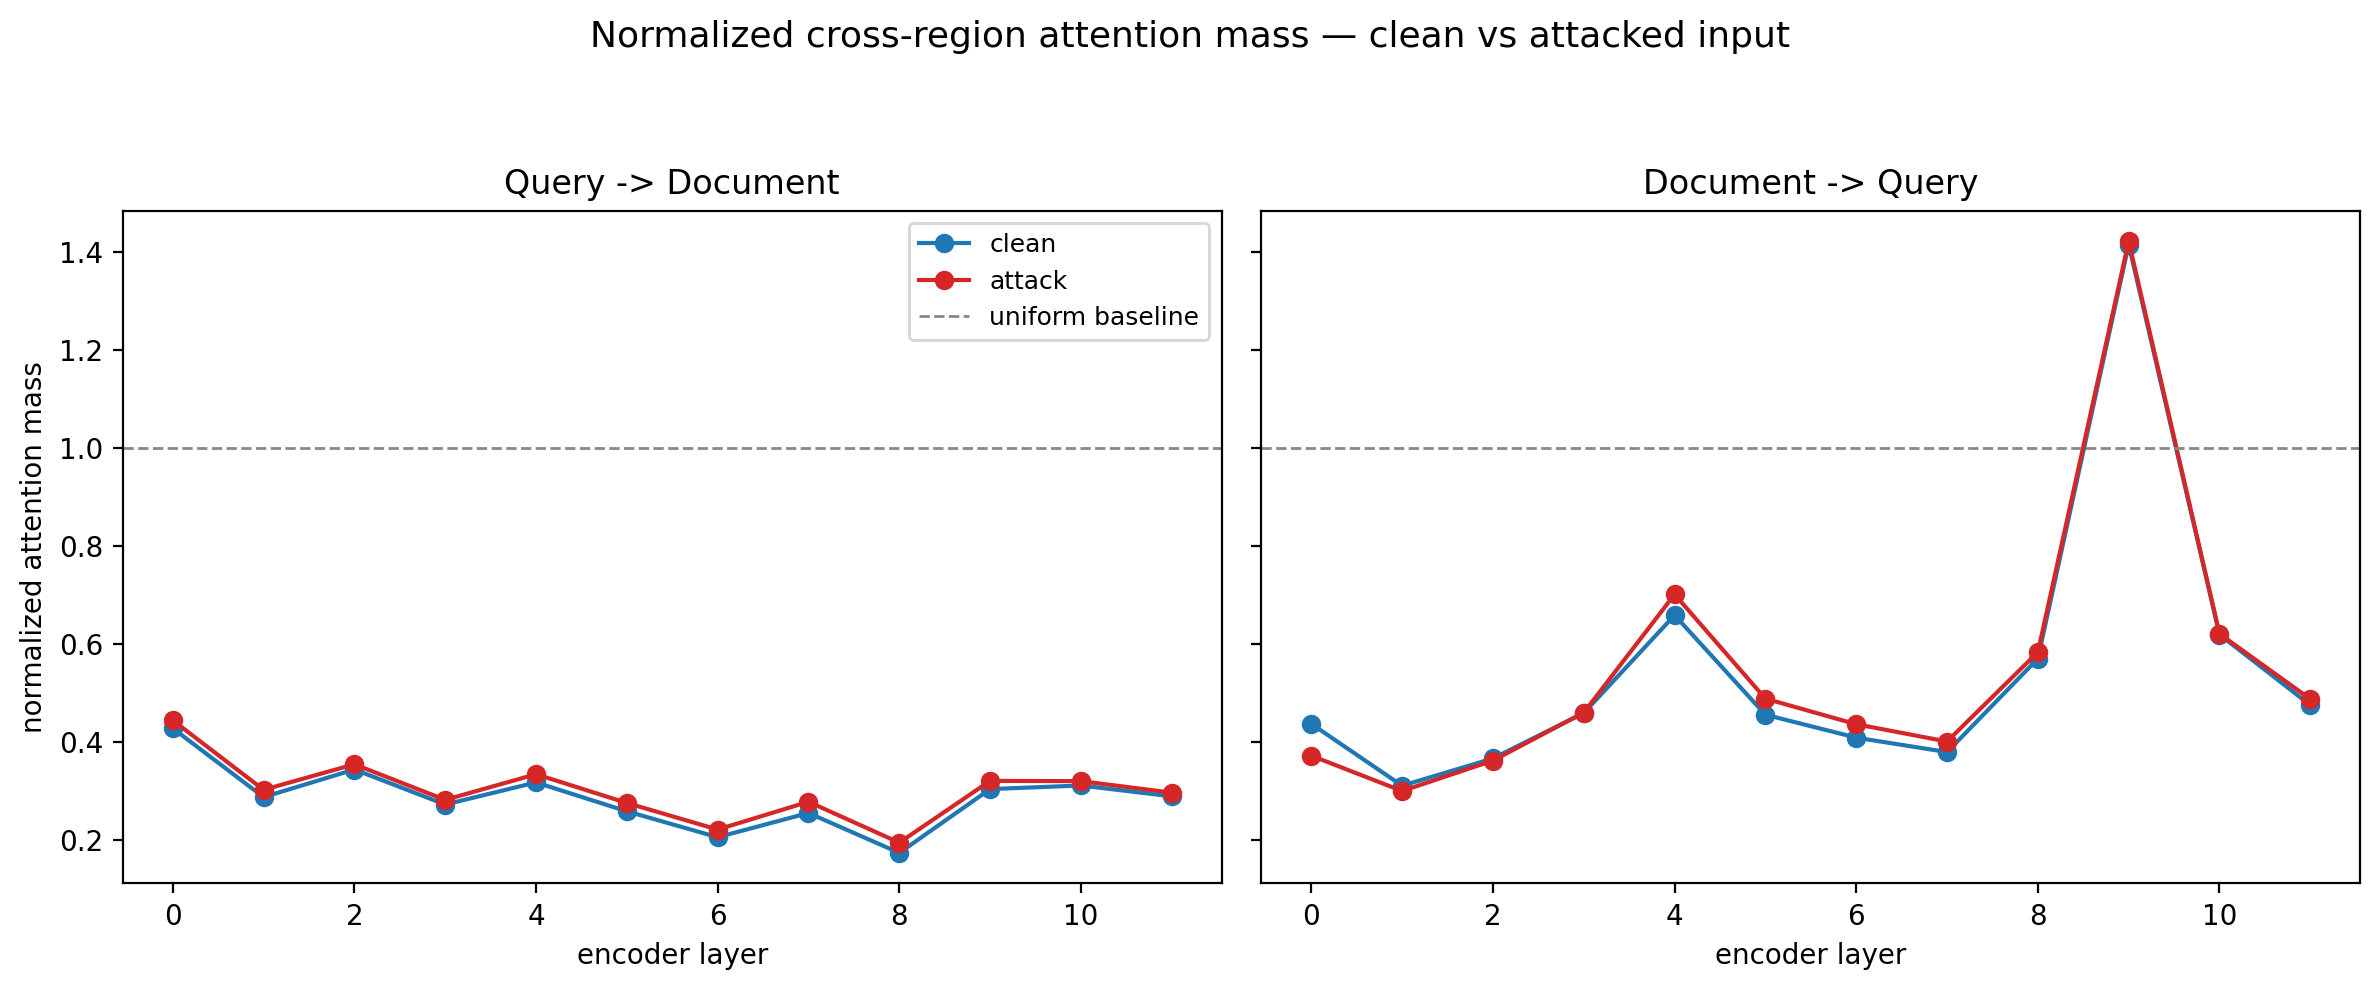
\includegraphics[width=0.95\textwidth]{outputs/plots/attention_mass_clean_vs_attack.png}
  \caption{Normalized attention mass per encoder layer, clean vs.\ attacked
  input, canonical attack ($n=100$). Left: query$\to$document. Right:
  document$\to$query. Dashed line: uniform-attention baseline (1.0).}
  \label{fig:attnmass}
\end{figure}

\paragraph{Query-to-document} mass sits consistently \emph{below} the
uniform baseline at every layer ($0.17$--$0.43$), meaning individual query
positions do not preferentially attend to the document more than their
token-count share would predict — but the attack consistently
\emph{increases} it slightly at every single layer (e.g.\ layer~8:
$0.173\to0.194$; layer~0: $0.428\to0.444$), a small but universal shift.

\paragraph{Document-to-query} mass is the more striking signal: mostly
in the $0.3$--$0.7$ range, but with a sharp, isolated spike at
\textbf{layer~9} — $1.42$ (clean) rising to $1.42$ (attack, effectively
unchanged in magnitude but already far above baseline) — meaning that at
this one layer, document positions attend to the (6-token) query span
\emph{more than 40\% above} what a uniform distribution would predict, an
anomaly relative to every neighbouring layer. Layer~4 shows a smaller
version of the same anomaly ($0.66\to0.70$). That this spike sits at
layer~9 — inside the 9--11 range where Experiments~1 and 3 independently
localise the attack's causal effect — is a suggestive, if descriptive,
alignment between where the document attends unusually strongly to the
query and where the attack's causal effect is strongest.

\subsection{The causal result: query-only patching moves the score, robustly, at late layers}

\begin{figure}[H]
  \centering
  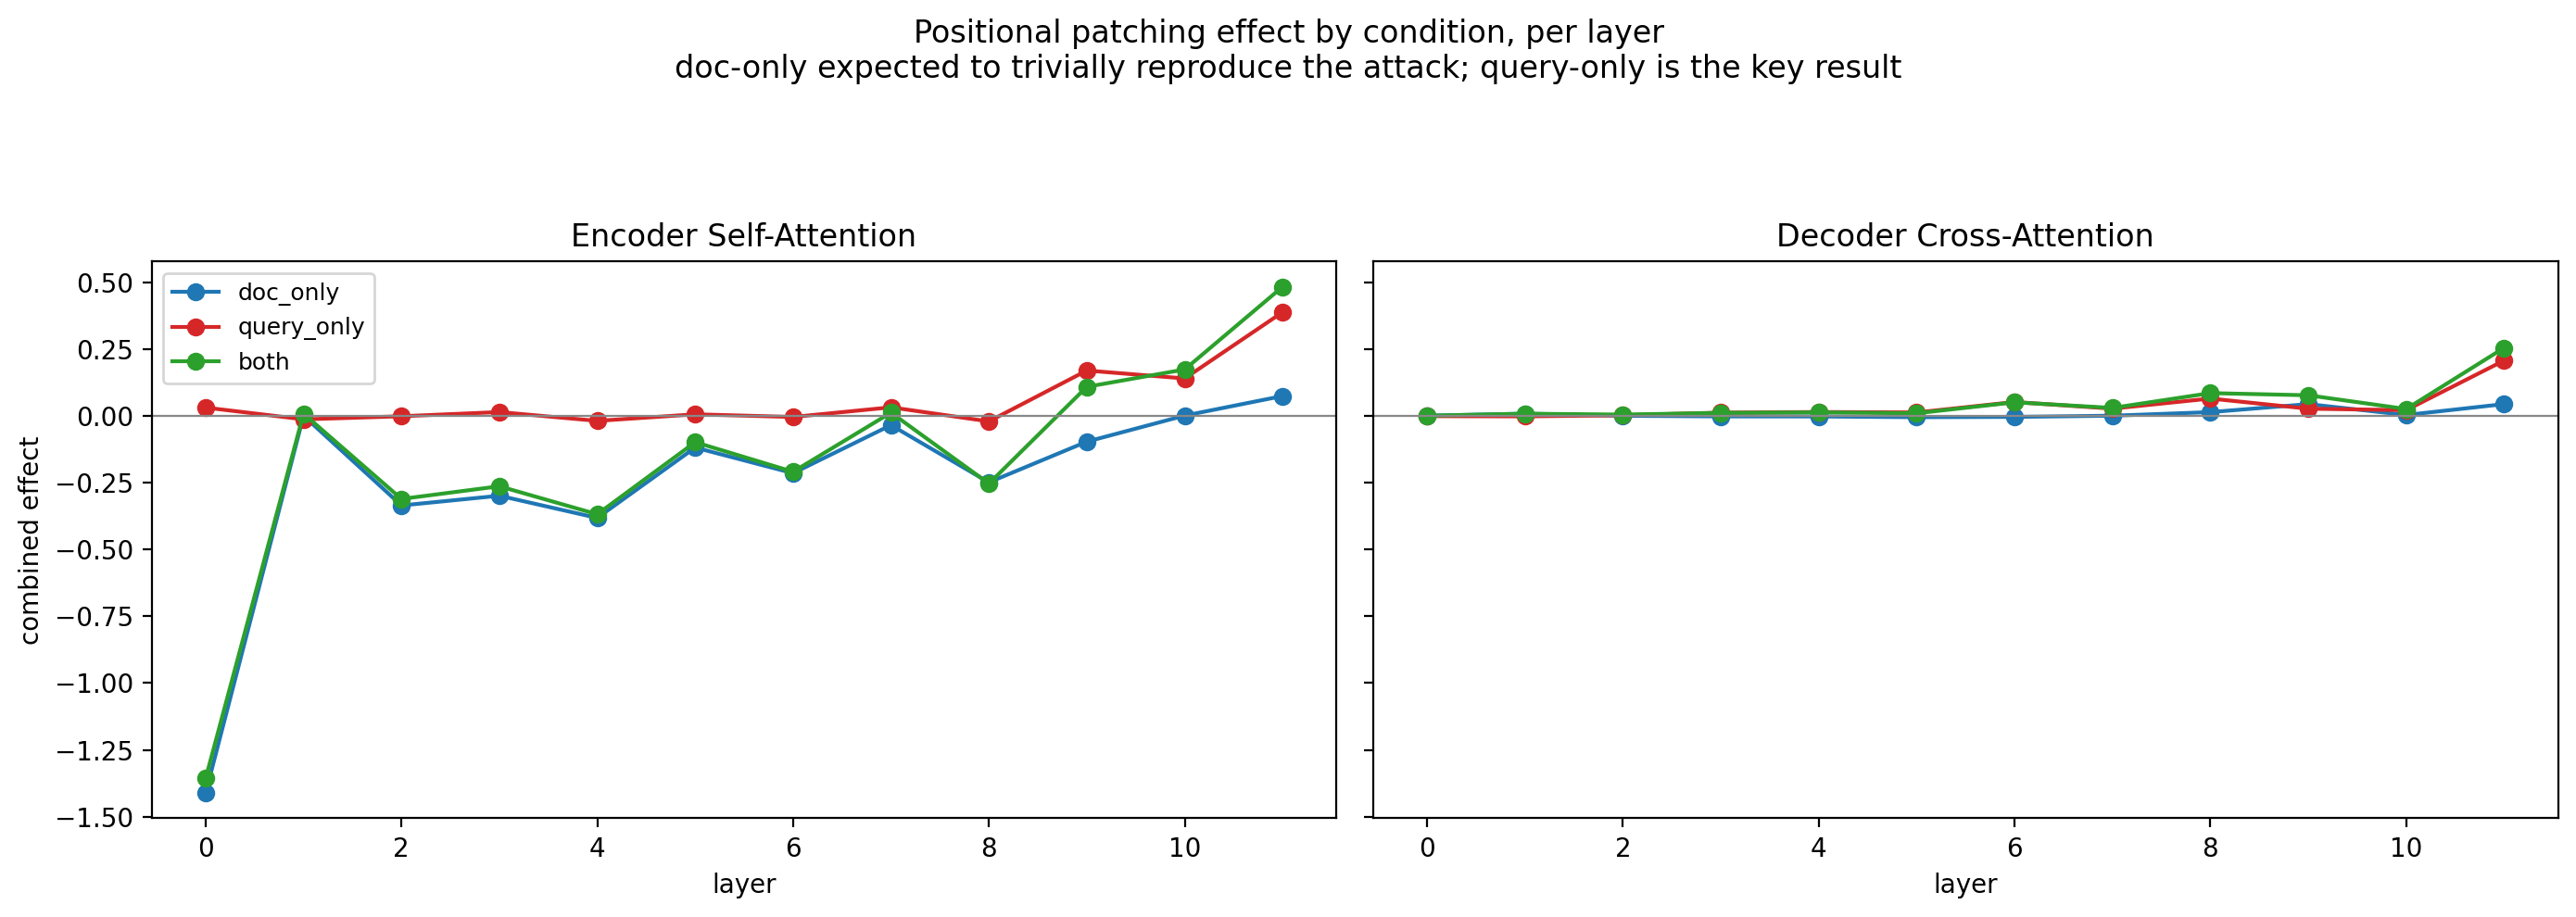
\includegraphics[width=0.95\textwidth]{outputs/plots/effect_by_condition.png}
  \caption{Combined patching effect per layer, one line per condition,
  encoder self-attention and decoder cross-attention side by side
  (canonical attack, $n=100$; means shown, see
  Section~\ref{sec:earlyinstability} for why medians are also reported in
  text for the encoder panel).}
  \label{fig:bycondition}
\end{figure}

\begin{table}[H]
\centering
\caption{Median combined effect, query\_only condition, canonical attack ($n=100$).}
\label{tab:queryonly}
\begin{tabular}{lrrrr}
\toprule
Region & Layer 0 & Layer 8 & Layer 9 & Layer 11 \\
\midrule
Encoder self-attention & 0.011 & 0.013 & 0.169 & \textbf{0.405} \\
Decoder cross-attention & $-$0.0002 & 0.073 & 0.032 & \textbf{0.191} \\
\bottomrule
\end{tabular}
\end{table}

Query-only patching is near-zero at early-to-mid layers for both regions
(median $|{\cdot}| < 0.03$ through layer~7 in encoder self-attention;
similarly small in decoder cross-attention through layer~5), then rises
sharply from layer~8/9 onward, peaking at layer~11 in both regions. This is
\textbf{the key result the experiment was designed to detect}: patching
\emph{only} the query positions' activations — swapping in what the encoder
computed for the query \emph{under the attacked document} — measurably
moves the final relevance score, and does so specifically in the same late
layers where the causal effect otherwise concentrates.

\paragraph{This is not a fluke of the canonical attack.} Repeating the same
measurement across the full 105-attack grid, encoder-layer-11 query-only
combined effect exceeds $0.2$ on \textbf{all 105 of 105 attacks} (range
$0.29$--$0.66$), and the grid's median trajectory (layers 0--11:
$0.02, 0.01, 0.02, 0.02, -0.01, 0.04, 0.01, 0.01, 0.07, 0.30, 0.36, 0.47$)
closely tracks the canonical attack's. Document$\to$query
cross-contamination in the late encoder is a universal property of this
attack family, not specific to one trigger word or position.

\begin{figure}[H]
  \centering
  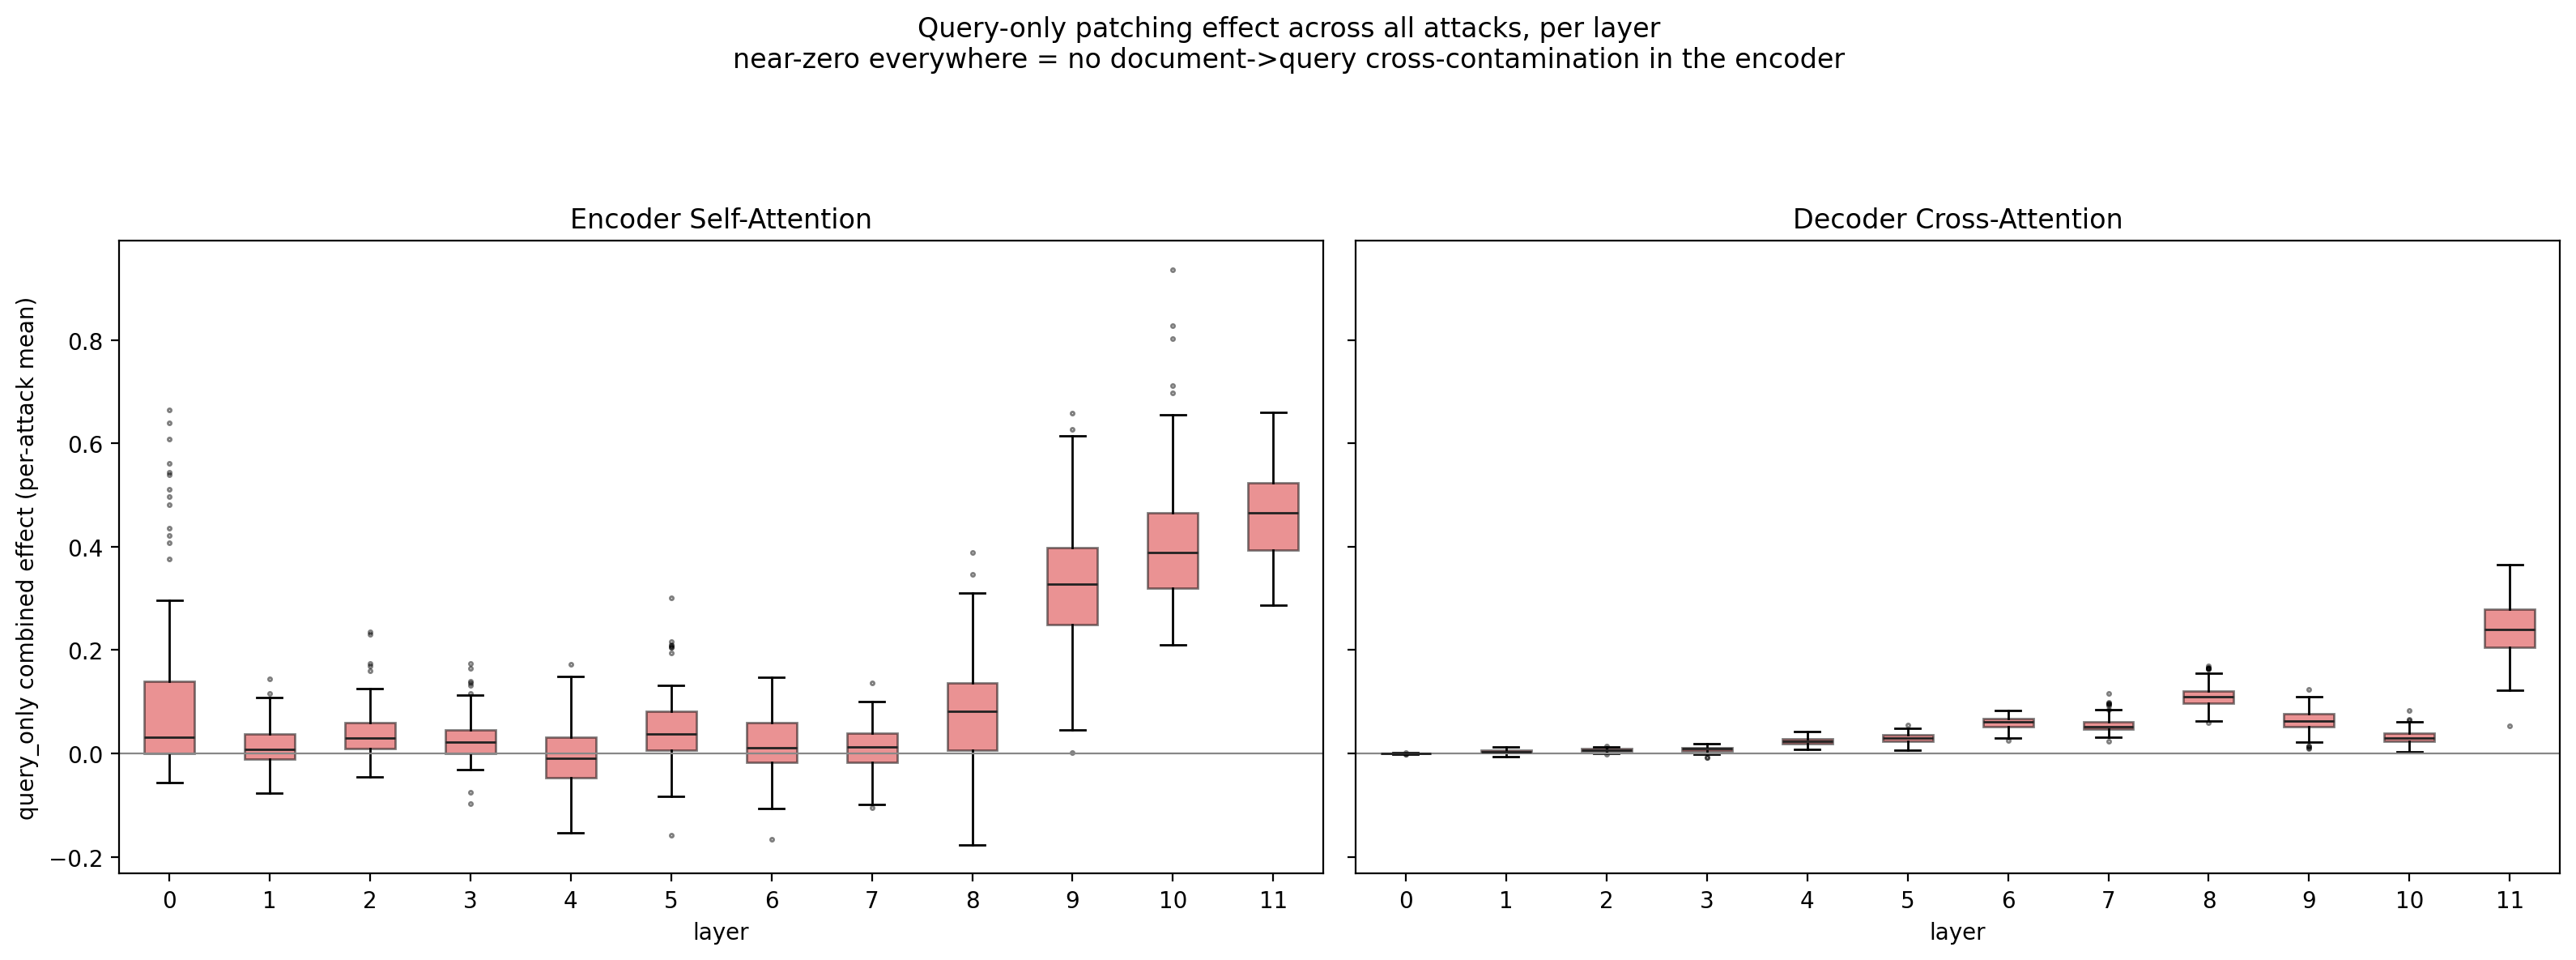
\includegraphics[width=0.95\textwidth]{outputs/plots/query_only_effect_across_attacks.png}
  \caption{Distribution of query-only combined effect across all 105
  attacks, per layer, encoder and decoder cross-attention. Both regions
  show the same late-layer rise seen in the canonical attack.}
  \label{fig:queryacrossattacks}
\end{figure}

\subsection{Document-only and ``both'': the early-layer instability}
\label{sec:earlyinstability}

Document-only patching was expected, a priori, to approximately reproduce
the whole attack (Section~\ref{sec:results} abstract) since the document
field contains every injected token. At \textbf{late} encoder layers this
holds in direction if not magnitude (layer~11 doc\_only median: $0.067$,
positive and in the expected direction, though smaller than Experiment~1's
whole-layer patch at the same layer, $0.687$ — see below for why). At
\textbf{early-to-mid} layers (0--8), however, both \texttt{doc\_only} and
\texttt{both} show large, often \emph{negative} median effects (e.g.\
layer~0: $-1.33$ and $-1.20$ respectively; layer~4: $-0.30$/$-0.28$) — an
overshoot past the control baseline in the wrong direction, not a mild
attenuation.

\paragraph{Diagnosis: this is a genuine consequence of the scope decision
to exclude connective positions, not a bug.} Two things were verified
directly. First, patching \emph{every} position (query $\cup$ document
$\cup$ the 9 excluded connective/EOS positions) at a given layer reproduces
Experiment~1's whole-layer patch exactly (e.g.\ layer~11,
$\fwd=0.598$ matches to 4 decimal places) — the patching mechanism itself
is correct. Second, the 9 excluded connective positions
(\texttt{"Query", ":", "Document", ":", "Relevant", "t", ":", "</s>"}, plus
a leading marker) carry $15$--$22\%$ of the total control-vs-attack
contribution-norm difference at a given layer, on real examples checked
directly — a real, non-negligible share. Leaving those positions at the
control run's own (different-from-attack) value while the query/document
positions now carry attack-derived contributions creates an internally
\emph{inconsistent} residual stream. At an early layer, this inconsistency
is then processed by \textbf{many more encoder layers}, which can amplify
or invert it before the final score is read out; by layer~11 there are no
more layers left to compound the inconsistency, so the effect is smaller
and correctly signed. Decoder cross-attention patches the encoder's output
just once, immediately before the single decoder step — there is no
"remaining layers to propagate through," and indeed its \texttt{doc\_only}
condition never shows this instability (Figure~\ref{fig:bycondition},
right panel: small and mostly non-negative at every layer).

\paragraph{Practical reading.} \texttt{doc\_only} and \texttt{both} should
be read as confirmatory only at the final 1--2 encoder layers; their
early-layer values reflect a real mechanistic property (partial-position
patching creates transient incoherence that propagates and can invert
sign) rather than the document field's causal importance, which is already
well established by Experiments~1 and 3. The \texttt{query\_only} results
above are unaffected by this caveat: they are consistently small and
correctly signed at every layer, growing smoothly rather than
discontinuously, which is itself evidence that the late-layer rise is a
real signal rather than an artefact of the same instability.

\subsection{Resolving the connective-position caveat: an extension experiment}
\label{sec:template-extension}

The Limitations section (originally) left one question open: the 9 excluded
connective positions carry 15--22\% of the contribution-norm difference at a
given layer (Section~\ref{sec:earlyinstability}), but were never causally
tested in isolation — only ever frozen (every condition above) or included
\emph{as part of the whole-layer sanity-check patch}. It was possible that
some of them are pure \textbf{attention sinks} (absorb mass, causally inert
when patched — which would mean freezing them was harmless) or that some
carry real \textbf{signal} (causally move the score when patched alone —
which would mean the \texttt{query\_only}/\texttt{doc\_only}/\texttt{both}
effect sizes above are underestimates).

\paragraph{Method.} Single-position causal patching (identical
forward/reverse/combined definitions, Eq.~4--6, encoder self-attention only)
of each of the 7 named template positions individually — the leading
SentencePiece space token folded together with \texttt{"Query"} (a
string-initial tokenization artefact, not a fourth region), the colon after
it, \texttt{"Document"}, its colon, the 2-subword \texttt{"Relevant"}
(\texttt{"Relevan"+"t"}, folded together), its colon, and \texttt{</s>} —
one position at a time, never combined. Positions are located per-example by
splitting the 3 gaps around \texttt{query\_span}/\texttt{doc\_span} on
decoded token content (never hardcoded offsets), verified robust across
examples ranging 74--207 tokens. Run on the canonical attack
(\texttt{relevant\_start\_5}, $n{=}100$, all 12 encoder layers) and,
unconditionally on all 7 positions (not pre-filtered by the canonical
result), across the full 105-attack grid ($n{=}10$/attack).

\begin{table}[H]
\centering
\caption{Template-position causal patch results. Peak = max mean
combined\_effect over layers 9--11 (canonical attack, $n=100$). Attacks
exceeding threshold ($>0.02$) out of 105. Peak incoming/outgoing = max
normalized attention mass (attack input, layers 9--11) into/out of the
position, from/to the document span. Classification per
Section~\ref{sec:template-extension}'s 2$\times$2 scheme.}
\label{tab:templatepositions}
\begin{tabular}{lrrrrl}
\toprule
Position & Peak $\comb$ & Attacks $>0.02$ & Peak in-mass & Peak out-mass & Class \\
\midrule
\texttt{"Query"}            & 0.072 & 91/105  & 2.57  & 4.22 & relay \\
\texttt{":"} (after Query)    & 0.053 & 105/105 & 3.35  & 4.92 & relay \\
\texttt{"Document"}         & 0.041 & 77/105  & 3.99  & 4.23 & relay \\
\texttt{":"} (after Document) & 0.035 & 89/105  & 5.08  & 4.48 & relay \\
\texttt{"Relevant"}         & 0.002 & 7/105   & 1.21  & 0.70 & sink \\
\texttt{":"} (after Relevant) & 0.006 & 5/105   & 2.29  & 1.15 & sink \\
\texttt{</s>}                & 0.002 & 0/105   & 40.02 & 0.75 & sink \\
\bottomrule
\end{tabular}
\end{table}

\begin{figure}[H]
  \centering
  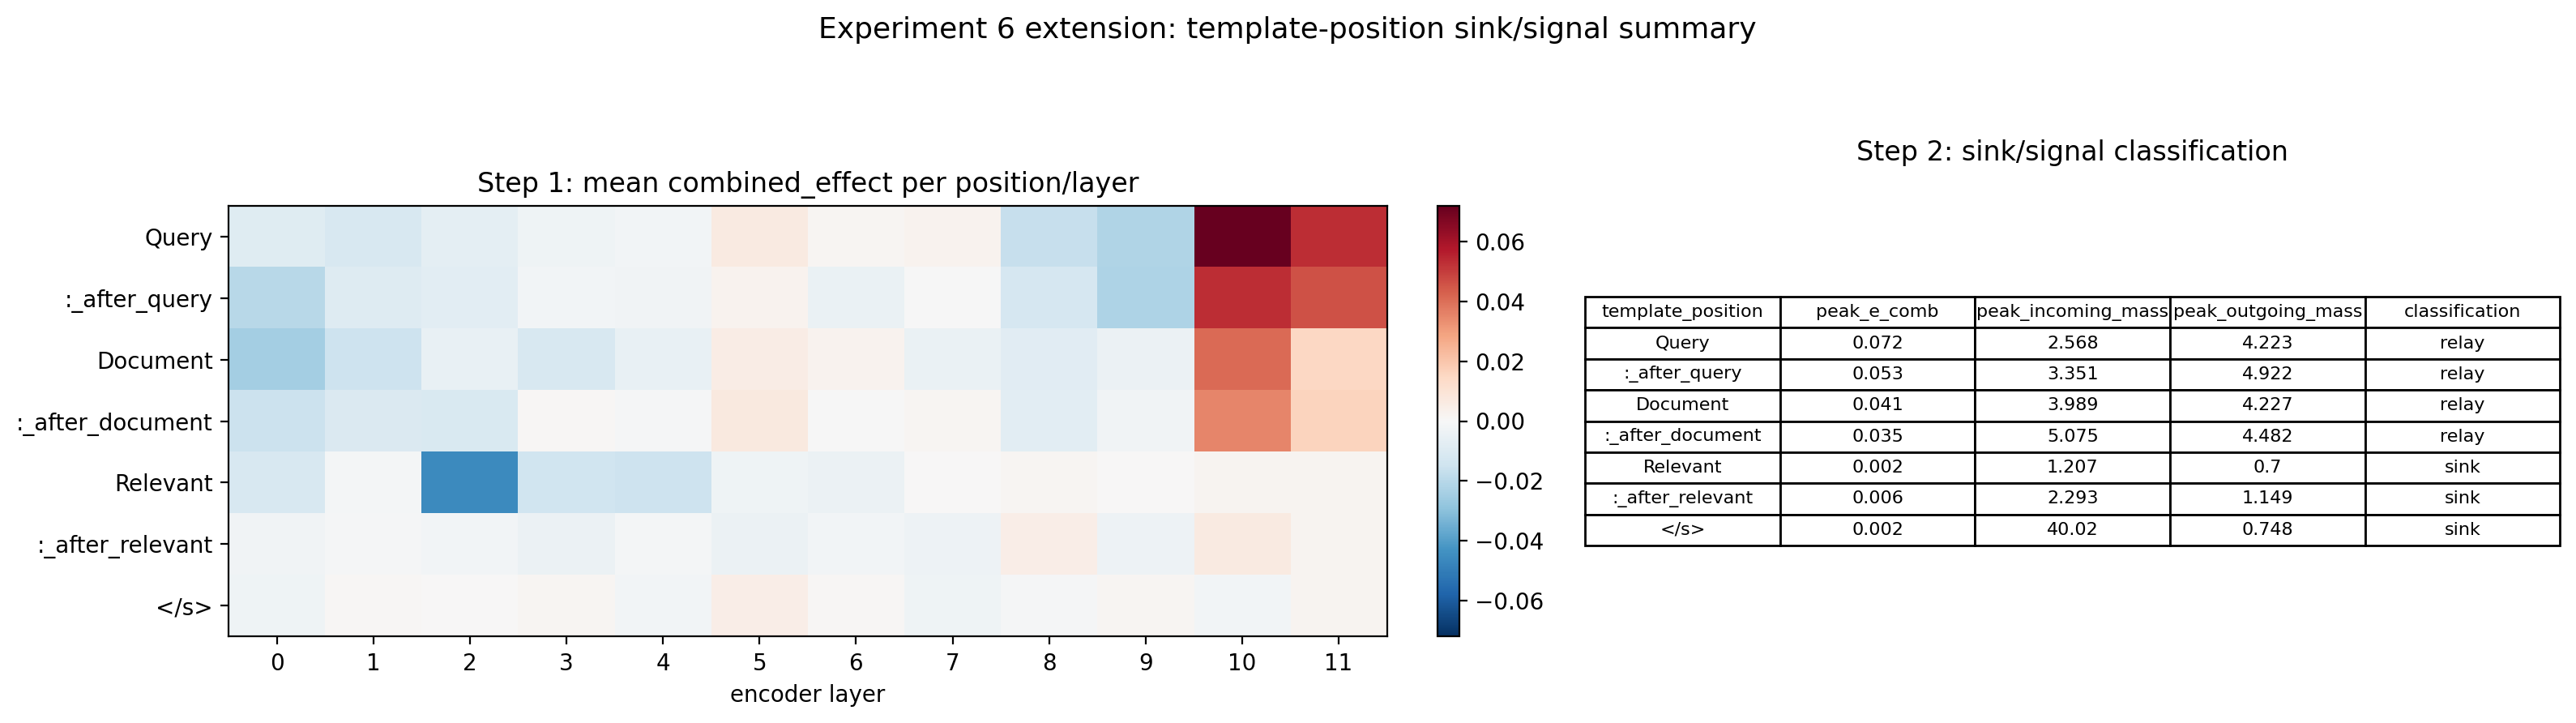
\includegraphics[width=0.95\textwidth]{outputs/template_tokens/plots/template_position_summary_figure.png}
  \caption{Left: mean combined\_effect per template position, per encoder
  layer (canonical attack, $n{=}100$). Right: the classification table
  above. Query/Document markers and their colons rise sharply at
  layers~10--11, matching the whole-query-span pattern; Relevant/its
  colon/\texttt{</s>} stay flat at every layer.}
  \label{fig:templateheatmap}
\end{figure}

\paragraph{Result: the caveat was real for 4 of 7 positions, not for the
other 3.} \texttt{"Query"}, \texttt{"Document"}, and the colon immediately
following each classify as \textbf{relay}: high attention mass (both
directions, matching or exceeding the whole document/query spans' own mass
in Table~\ref{tab:queryonly}) \emph{and} a non-trivial, robust causal effect
— flagged on 77--105 of 105 attacks, not just the canonical one
(Figure~\ref{fig:templateheatmap}, box-plot corroboration in
\texttt{outputs/template\_tokens/plots/template\_position\_sweep\_boxplots.png}
shows the same layers-10--11 rise pooled across the full grid, tight
interquartile ranges, no comparable rise for the sink positions). This
falsifies the sink hypothesis for these 4 positions and confirms it for the
remaining 3: \texttt{"Relevant"}, its colon, and \texttt{</s>} all have
peak $\comb \le 0.006$, flagged on at most 7/105 attacks — and \texttt{</s>}
in particular has by far the highest incoming mass of any position tested
(40.0$\times$ uniform, the expected behaviour of a T5 attention sink given
the model has no BOS token) while being \emph{the least} causally important
position measured, the cleanest possible sink signature.

\paragraph{Additivity (Step 3 check).} Summing the 7 positions' individual
peak effects gives $0.211$, against $0.484$ for the existing whole-span
\texttt{both} (query$\cup$document) condition's peak at the same layers —
a ratio of $0.44\times$, sub-additive. This does \emph{not} mean "the true
query/document effect is $0.484 + 0.211$"; positions interact (consistent
with Section~\ref{sec:earlyinstability}'s finding that partial-position
patches are not simply separable), so the individual-position numbers
should be read as proof that the excluded positions carry independent,
non-negligible signal, not as an additive correction term.

\paragraph{Consequence for the rest of this report.} The
\texttt{query\_only}/\texttt{doc\_only}/\texttt{both} effect sizes reported
in Section~\ref{sec:results} (including the abstract's ``$>0.2$ on 105/105
attacks'' claim) are computed with \texttt{"Query"}/\texttt{"Document"} and
their colons frozen at the control value in every condition. Since those
4 positions independently move the score at the same layers (9--11) via
presumably the same document$\to$query mixing mechanism, the reported
effect sizes \textbf{understate} the true query/document pathway's
magnitude — by how much is not resolved here (the sub-additivity above
means simple summation overstates the correction), but the direction is
unambiguous: this report's headline numbers are a lower bound, not a point
estimate. Reproduction: \texttt{bash bash/run\_template\_tokens.sh
configs/template\_tokens.yaml} (SLURM: 100 canonical + 1{,}050 grid
examples $\times$ 12 layers $\times$ 7 positions $=$ 96{,}600 rows, zero
alignment failures, $\approx$62~minutes wall-clock on 1$\times$ L40); full
outputs and the written per-position verdict in
\texttt{outputs/template\_tokens/SUMMARY.md}.

% =====================================================================
\section{Overall Interpretation and Discussion}
% =====================================================================

\begin{enumerate}
  \item \textbf{The encoder mixes document information into the query's
  representation, specifically in the late layers.} Query-only patching
  at encoder layer~11 moves the score substantially and universally
  (105/105 attacks, effect $>0.2$). Combined with Experiments~1 and 3's
  finding that the causal effect and the important heads both concentrate
  in layers 9--11, this suggests a single mechanistic story: by the time
  the encoder finishes, the attack has not just corrupted the document's
  own representation — it has corrupted the query's too, at the same
  layers, via the same self-attention mechanism. This effect size is a
  \emph{lower bound}: Section~\ref{sec:template-extension} shows the
  \texttt{"Query"}/\texttt{"Document"} template markers (frozen out of this
  patch by construction) independently move the score at the same layers.
  \item \textbf{A descriptive anomaly (layer-9 document$\to$query
  attention mass) lines up with the causal finding.} The attention-mass
  spike at layer~9 (document attends to query 42\% above baseline) is not,
  by itself, evidence of anything causal, but its co-location with the
  onset of the query-only patching effect is a natural place to look next
  with per-head granularity (out of scope this pass).
  \item \textbf{Position-restricted patching at early layers is
  qualitatively different from whole-layer patching}, in a way that is
  easy to misread as a bug. Excluding even a small set of connective
  positions from a patch, at a layer with many remaining layers to
  process the result, can produce large, sign-flipped effects that have
  nothing to do with the excluded region's importance and everything to
  do with residual-stream incoherence. Any future per-position patching
  study should report effects layer-by-layer, not just at the final layer,
  and should not assume the sanity-check condition will trivially reproduce
  the whole-network number outside the last 1--2 layers.
  \item \textbf{Decoder cross-attention is the cleaner region for
  positional patching.} Because it intervenes once, immediately before
  the single decoder step, it does not suffer the encoder's
  propagation-instability problem, and its \texttt{query\_only} /
  \texttt{doc\_only} curves are monotonic and interpretable at every layer.
  \item \textbf{Not all excluded connective positions are equal.}
  Section~\ref{sec:template-extension}'s extension experiment causally
  tested all 7 template positions individually: \texttt{"Query"},
  \texttt{"Document"}, and their colons are signal-carrying (robust across
  77--105/105 attacks), while \texttt{"Relevant"}, its colon, and
  \texttt{</s>} are genuine sinks (\texttt{</s>} has the highest attention
  mass of any position tested, $40\times$ uniform, yet the lowest causal
  effect). "Connective token" was doing too much work as a single category
  -- some connective tokens are load-bearing for the query/document mixing
  mechanism, others are inert absorbers, and the two cannot be told apart
  without a per-position causal test.
\end{enumerate}

% =====================================================================
\section{Limitations and Threats to Validity}
% =====================================================================

\begin{itemize}
  \item \textbf{Connective positions are never patched -- now causally
  tested, not just quantified.} By construction, 9 positions (the literal
  template markers and EOS) are excluded from all three conditions in every
  layer. Section~\ref{sec:earlyinstability} quantifies their share of the
  contribution difference (15--22\%); Section~\ref{sec:template-extension}'s
  follow-up experiment resolves what that share means causally: 4 of the 7
  named positions (\texttt{"Query"}, \texttt{"Document"}, and the colon
  after each) are \textbf{not} inert -- they move the score independently
  at layers 9--11, robust across 77--105 of 105 attacks -- so this report's
  \texttt{query\_only}/\texttt{doc\_only}/\texttt{both} effect sizes are
  confirmed \textbf{lower bounds}, not the complete pathway. The other 3
  (\texttt{"Relevant"}, its colon, \texttt{</s>}) test as genuine sinks
  (peak $\comb \le 0.006$, flagged on at most 7/105 attacks), so freezing
  those specifically was harmless.
  \item \textbf{Whole-block only.} Per-head positional patching is out of
  scope this pass, matching Experiment~3's own per-head/whole-block
  scoping decision; the layer-9 attention-mass anomaly and the layer-11
  query-only effect are natural candidates for head-level follow-up.
  \item \textbf{Grid~A depth.} The 105-attack grid uses $n=10$/attack
  (unlike Experiments~3/6's later $n=100$ revisions); the query-only
  robustness claim (105/105 attacks $>0.2$ at layer~11) is nonetheless a
  strong signal since the effect size is large relative to the noise floor
  at this sample size.
  \item \textbf{Single model/dataset.} Results are for monoT5-base on
  DL19, matching Experiments~1, 3, and the rest of this project.
\end{itemize}

% =====================================================================
\section{Reproducibility}
% =====================================================================

From \texttt{06\_monot5\_query\_doc\_patching/}, with the
\texttt{advseq2seq} conda environment and Experiment~1's outputs present
as a sibling directory:

\begin{lstlisting}
bash bash/run_tests.sh          # unit tests (real tokenizer + tiny random T5, CPU)
bash bash/run_pilot.sh          # timing pilot
bash bash/run_all.sh            # full pipeline (resume-safe)
bash bash/run_template_tokens.sh  # extension: template-position sink/signal (Sec.~\ref{sec:template-extension})
\end{lstlisting}

\noindent On this run: SLURM job on 1$\times$ L40 GPU, $\approx$50~minutes
wall-clock for both runs plus aggregation and plotting; outputs under
\texttt{outputs/\{grid,canonical\}/} and \texttt{outputs/plots/}. The
extension experiment (separate SLURM job) took $\approx$62~minutes on the
same GPU type; outputs under \texttt{outputs/template\_tokens/}.

% =====================================================================
\section*{Appendix: Glossary of Key Quantities}
\addcontentsline{toc}{section}{Appendix: Glossary of Key Quantities}
% =====================================================================

\begin{description}[leftmargin=1.6em,style=nextline]
  \item[normalized\_mass$(A\to B)$] attention mass from region $A$ to
  region $B$, normalised by $B$'s share of total sequence length,
  Eq.~\eqref{eq:attnmass}. $>1$ means more attention than a uniform
  baseline predicts.
  \item[query span / document span] token-index ranges for the query text
  and the entire document field (attack tokens included), alignment-checked
  against the prompt template.
  \item[doc\_only / query\_only / both] which span's positions get the
  attack run's contribution patched into the control run.
  \item[$\fwd$ / $\rev$ / $\comb$] forward/reverse/combined patching
  effect, identical formulas to Experiment~1, applied per (layer,
  condition).
  \item[early-layer instability] the large, sometimes sign-flipped
  \texttt{doc\_only}/\texttt{both} effects at encoder layers 0--8,
  explained in Section~\ref{sec:earlyinstability}.
\end{description}

\end{document}
